\documentclass[Rapport/Rapport_main.tex]{subfiles}

\begin{document}

\subsection{Cup Sensor}
Lyset for hvert CupLight skal i UC1 og UC2 styres på baggrund af, om der er placeret en kop, og i UC2 også om en bold er ramt i en kop. Derudover skal RPi vide hvilke kopper, der er placeret på en given playerside, da den skal vide, hvornår spillet er færdigt.
\subsubsection{Hardwaredesign}
For at detektere placering af en kop, og at bold rammer i en kop, er der udført en teknologiundersøgelse (afsnit \fullref{hwdesign:sec:CupSensorTekUnder} i Hardwaredesign bilaget). I denne undersøgelse, overvejes forskellige egenskaber en kop med øl har, som kan måles. Det overvejes bl.a., at koppen har en masse, koppen påvirker lys, og koppen har en anden dielektricitetskonstant end luft. Der undersøges i detalje sensorer, der måler de to sidste egenskaber, en kapacitiv sensor og en optisk sensor. Disse to sensorer sammenlignes og bl.a., fordi den optiske sensor viste bedste tegn til at detektere, at en bold rammer i, vælges denne metode, på trods at et lavere signal-støjforhold.

\begin{figure}[H]
    \centering
    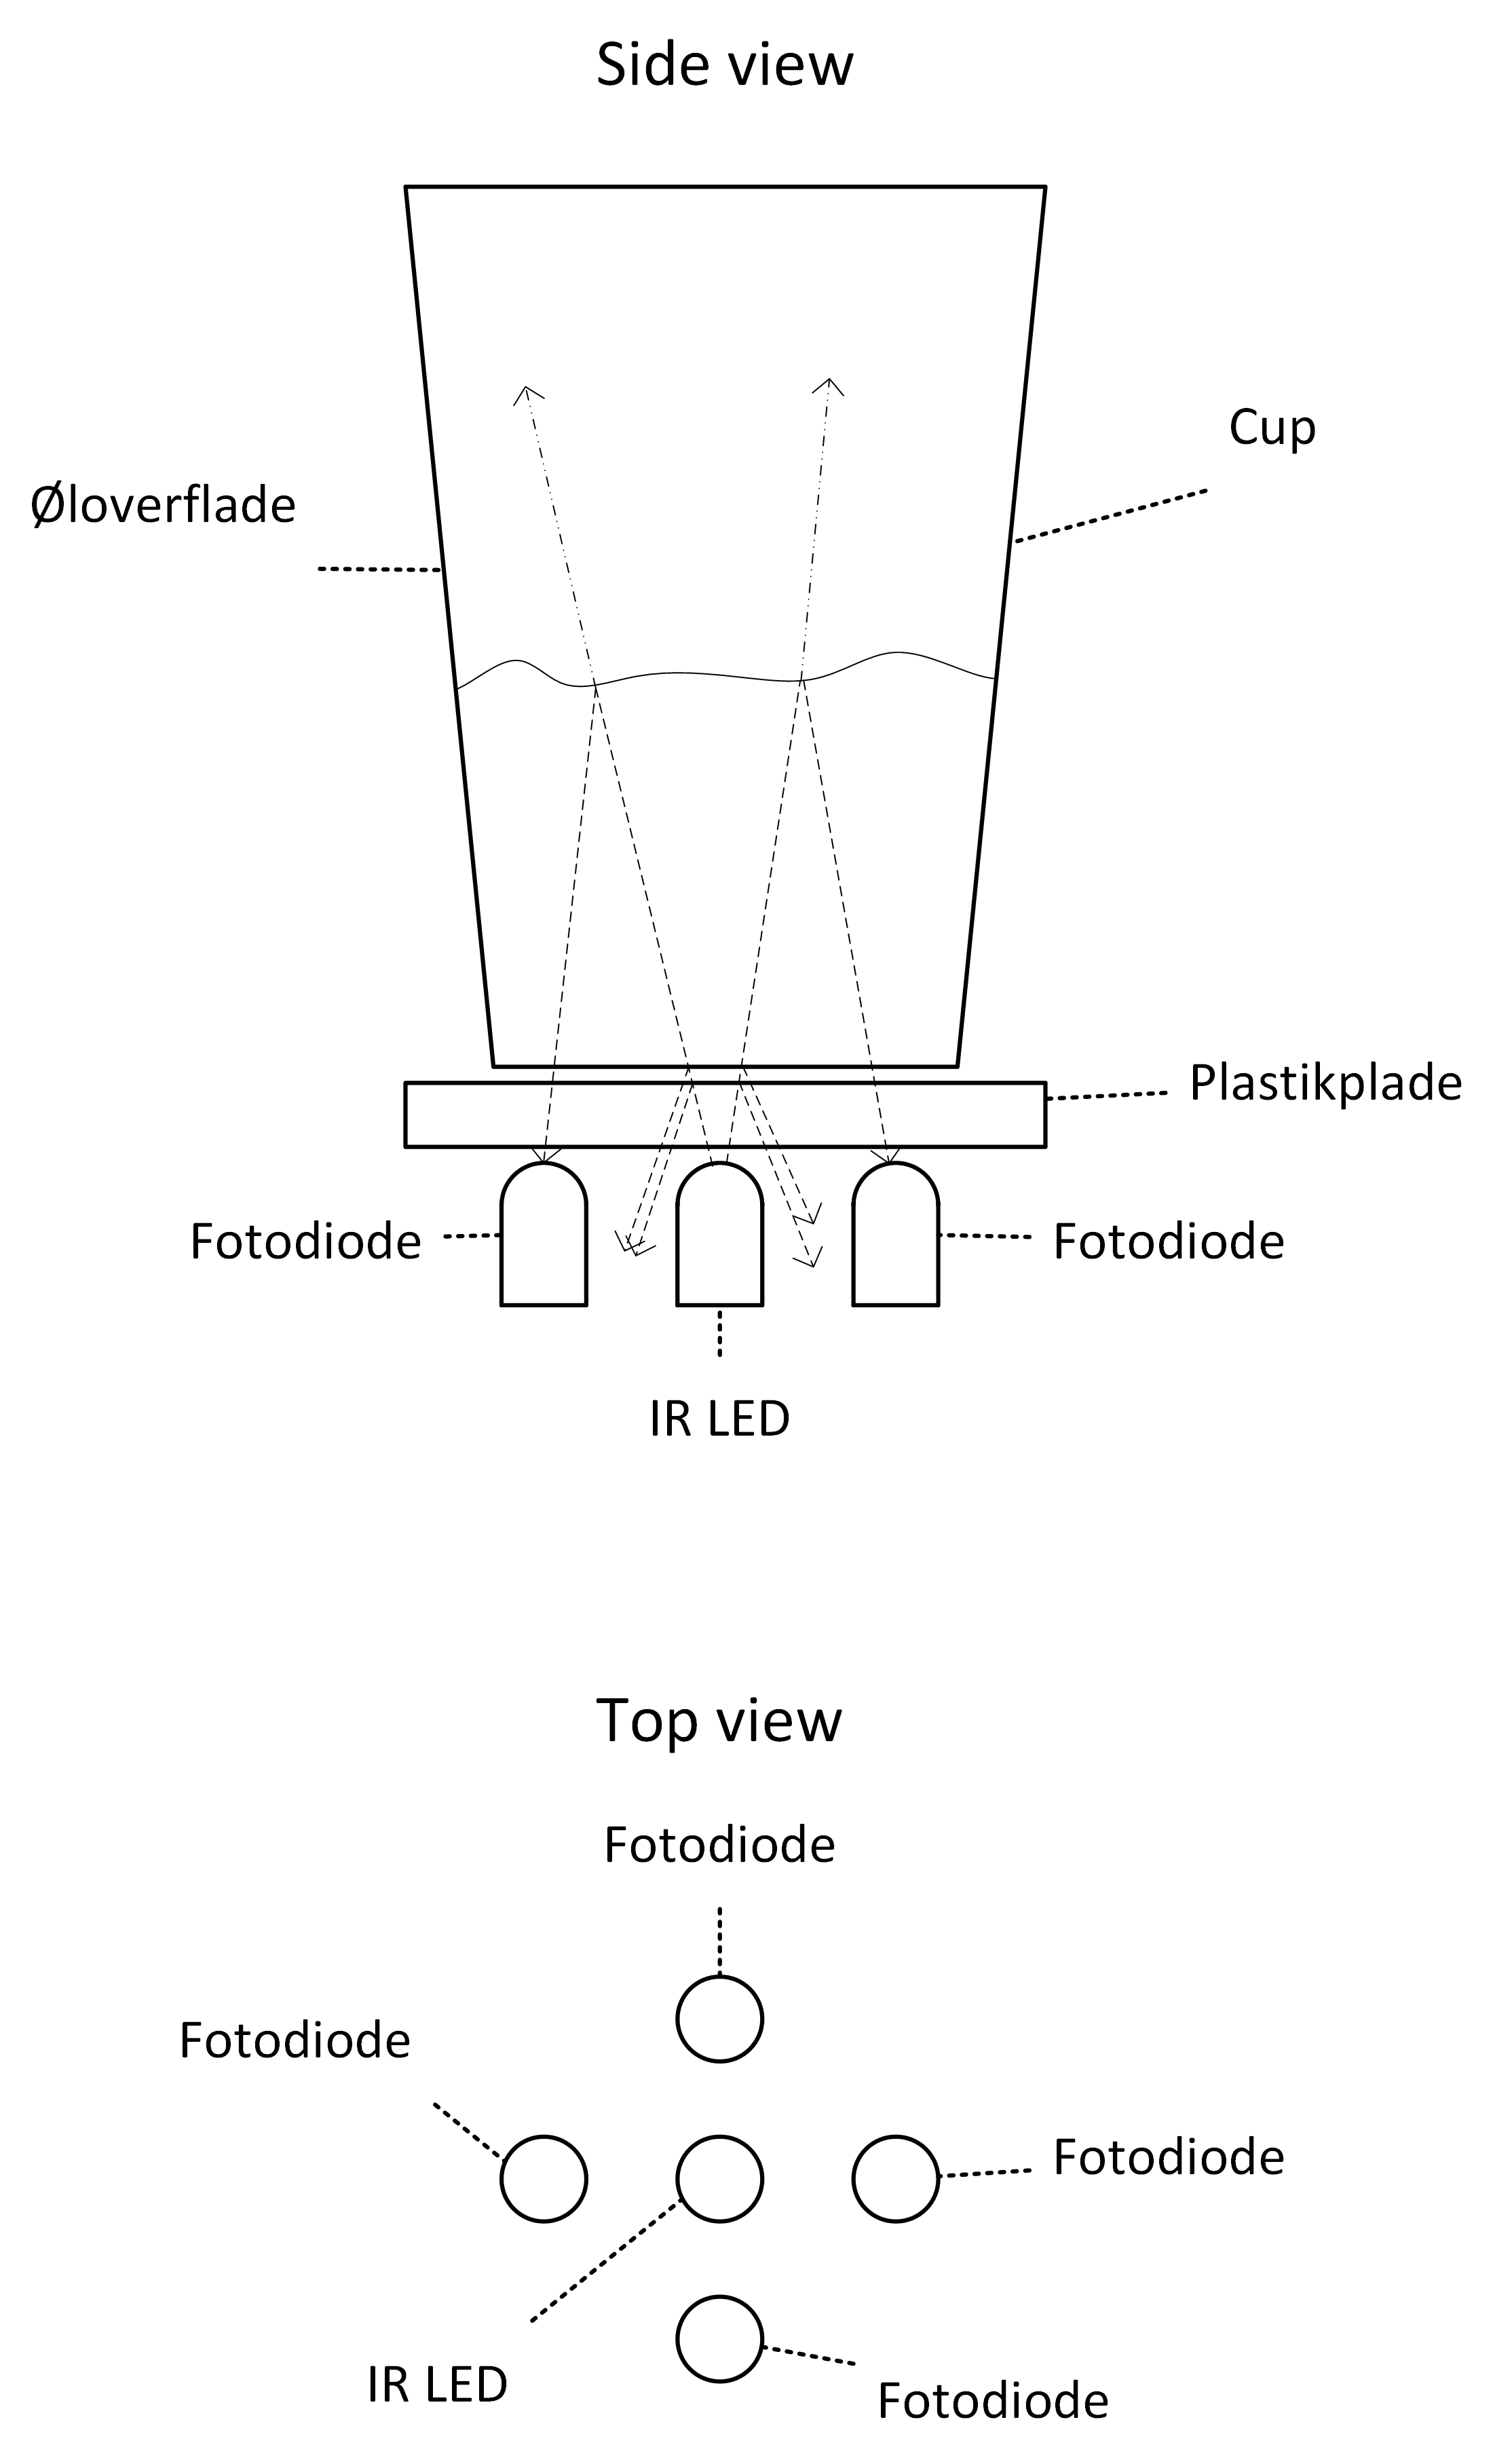
\includegraphics[width=0.8\textwidth]{HardwareDesign/CupSensor/graphics/lightPath.png}
    \caption{Her ses hvordan opstillingen af sensoren skal være. Både fra siden og fra toppen. Der benyttes én IR LED, og fire fotodioder. Der er derudover tegnet Cup med øl og gennemsigtig plastikplade på skitsen. Der er også påtegnet, hvordan det tænkes, lyset vil bevæge sig}
    \label{fig:lightPaht}
\end{figure}

For at lave en optisk sensor benyttes der opstillingen, som ses på \ref{fig:lightPaht}. Der benyttes en IR LED, som lyser op i centrum af koppen og 4 fotodioder, som er sensitive over for det lys, som LED'en udsender. På baggrund af teknologiundersøgelsen benyttes der 4 fotodioder, og det findes at den optimale afstand mellem en LED og en fotodiode er ca. 10mm. Kredsløbet kan ses på figur \ref{fig:CupSensorDesign}.
\begin{figure}[H]
    \centering
    \makebox[\textwidth][c]{%
        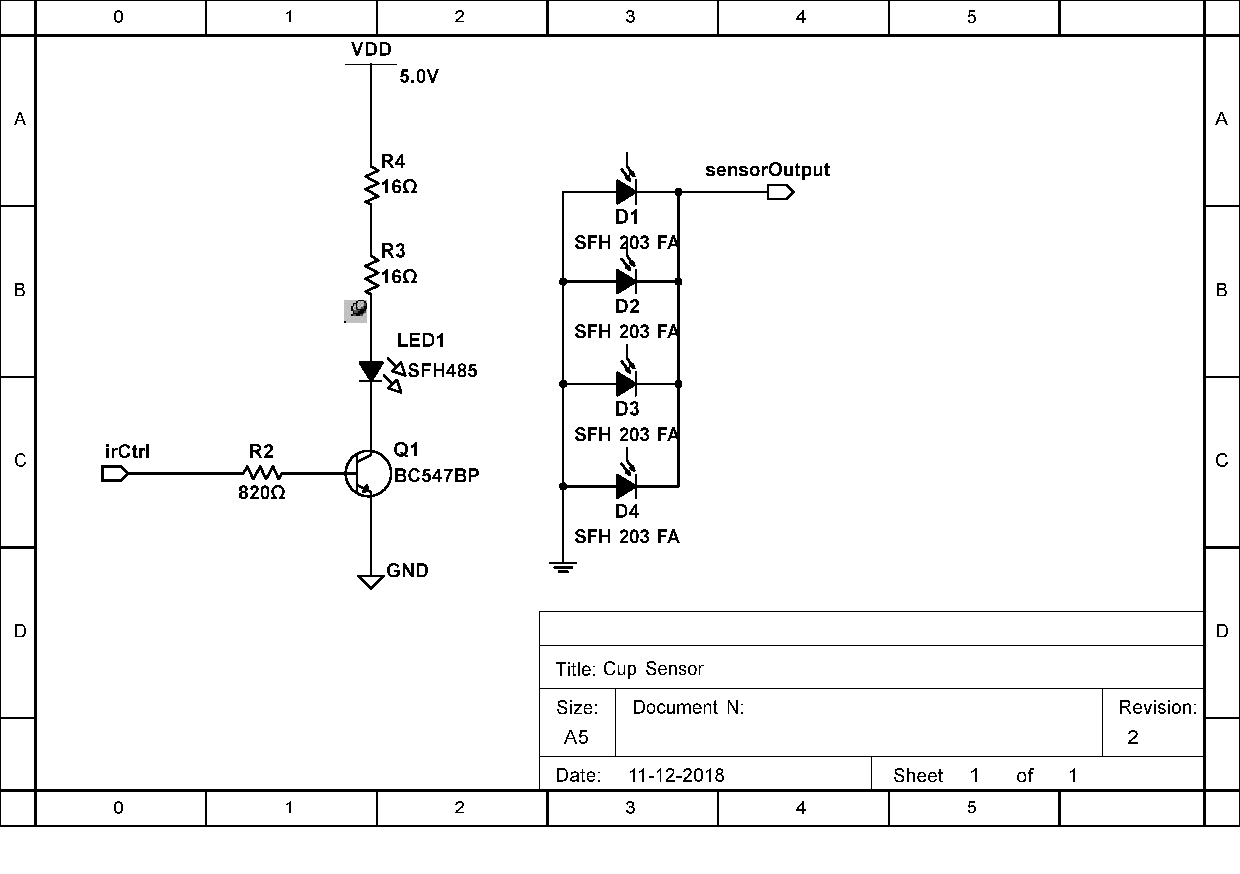
\includegraphics[width=1\columnwidth,trim={0.6in 1.8in 2.6in 0.25in},clip, page=1]{HardwareDesign/CupSensor/graphics/FinalDesign/CupSensor.pdf}
    }
    \caption{Design af Cup Sensor.}
    \label{fig:CupSensorDesign}
\end{figure}
Fotodioder virker på den måde, at der i spærreretningen løber en strøm afhængig af lysintensiteten. Omgivelserne kan variere meget, og der kommer et DC-offset, hvis systemet fx bruges udendørs i sollys. Derfor er det valgt at blinke med LED'en, som styres vha. 'irCtrl', og nyttesignalet er derfor et AC-signal. Til at sortere DC'en væk, bruges et højpasfilter som er en del af Cup Holder Controller. Alle 6 Cup Sensor's forbindes til dette filter. (se afsnit \ref{hwdesign:sec:CupSensor} i bilaget \textbf{Hardwaredesign}). 
Derudover benyttes der på PSoC'en en TIA til at konvertere strømsignalet til en spænding. Vha. mixerfunktionalitet indbygget i en Delta Sigma ADC laves der et båndpasfilter med centerfrekvens på $10\si{kHz}$ og 3dB båndbredde på $1.138\si{kHz}$ 

PSoC Komponenten kan ses på figur \ref{fig:CupSensorPSoCDesign}. Det ses, at der bruges en demultiplexer, hvor hvert output ledControl0, ledControl1 ..., styrer LED'en på hver Cup Sensor. På denne måde kan det vha. Control\_Red\_Led styres hvilken Cup Sensor's LED, der skal blinke, og dermed modtages der kun signalet fra denne sensor, selvom alle fotodioderne er forbundet til hinanden.  

\begin{figure}[H]
    \centering
    \makebox[\textwidth][c]{%
        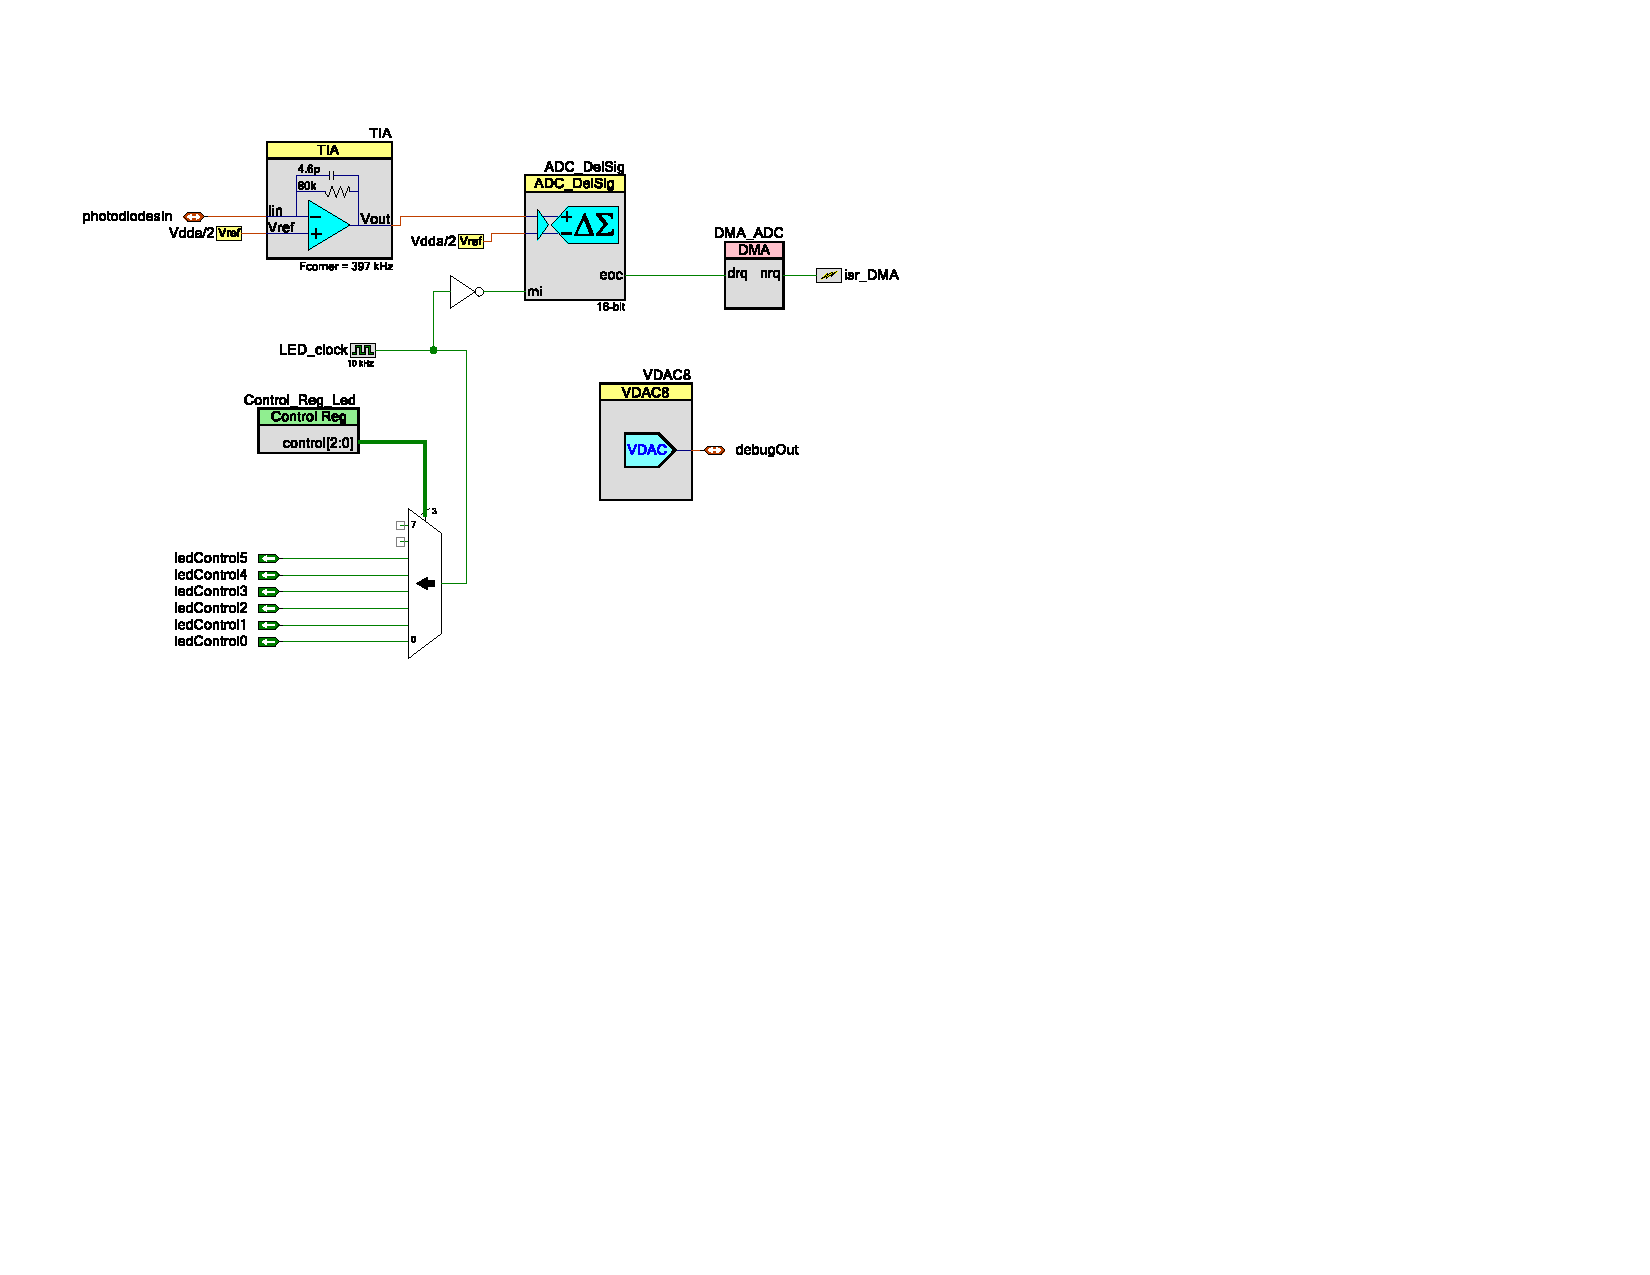
\includegraphics[width=1\columnwidth,trim={0.5in 4.1in 4.5in 0.8in},clip, page=1]{HardwareDesign/CupSensor/graphics/FinalDesign/PSoC-design.pdf}
    }
    \caption{PSoC design. 'photodiodesIn' forbindes til et højpasfilter}
    \label{fig:CupSensorPSoCDesign}
\end{figure}

\subsubsection{Softwaredesign}
Der er til softwaredesign af CupSensor\_IF, udviklet et klassediagram. Diagrammet kan ses på figur \ref{fig:CupSensor-IF-classDiagram}.  Klassen CupSensor\_IF er den klasse, som GameController interagerer med. De resterende klasser er en del af en custom component i PSoC, se afsnit \ref{sec:CupSensorImplementering}. CupSensor er hovedklassen, som har en ISR som kaldes, når der kommer en ny måling fra ADC'en. 
 
\begin{figure}[H]
    \centering
    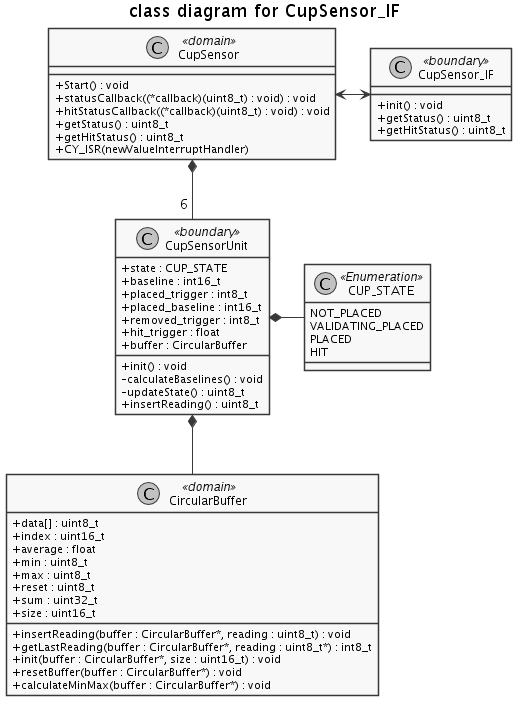
\includegraphics[width=0.8\textwidth]{Softwaredesign/CupSensor_IF/graphics/classDiagram.png}
    \caption{Klassediagram for softwaren til CupSensor\_IF.}
    \label{fig:CupSensor-IF-classDiagram}
\end{figure}

Der er 6 objekter af klassen CupSensorUnit. Denne repræsenterer hver Cup Sensor. Hver CupSensorUnit har en CUP\_STATE til at holde styr på tilstanden af den givne Cup Sensor. Derudover er der en CircularBuffer klasse, som bruges til at lagre de seneste målinger for hver CupSensorUnit.

Til at styre tilstanden for CupSensorUnit udvikles en tilstandsmaskine, som ses på figur \ref{fig:CupSensor-IF-state}. Der modtages en for hver 'reading', som evalueres i tilstandsmaskinen. Modtagelsen af denne reading mm. kan ses i \fullref{swdesign:sec:CupSensorSWDesign} i Softwaredesign bilaget.

\begin{figure}[H]
    \centering
    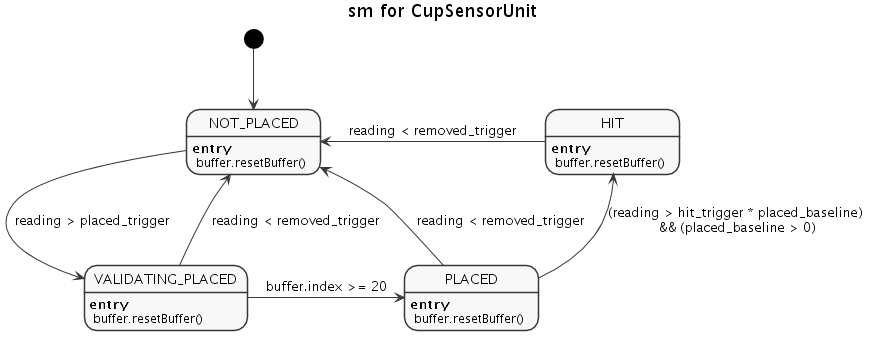
\includegraphics[width=1\textwidth]{Softwaredesign/CupSensor_IF/graphics/state.png}
    \caption{Tilstandsmaskine til CupSensorUnit.}
    \label{fig:CupSensor-IF-state}
\end{figure}

Til at bestemme de forskellige grænseværdier er der udført nogle målinger, hvor der placeres/fjernes en kop flere gange, og der tabes en bold flere gange. Dette udføres med forskellige mængder øl. Målinger og argumentation for valg af grænseværdier kan ses i \fullref{swdesign:sec:CupSensorThresholds} i Softwaredesign bilaget. 

 

\subsubsection{Implementering}\label{sec:CupSensorImplementering}
Der er valgt at lave en custom PSoC komponent kaldet CupSensor (afsnit \fullref{hwdesign:sec:CupSensorFinalDesign} i \textbf{Hardwaredesign} bilaget). Det implementeres som 'objektorienteret C' (afsnit \fullref{swdesign:sec:CupSensorImplementation} i \textbf{Softwaredesign} bilaget)

\subsubsection{Modultest}
I modultesten testes sensoren ud fra de krav, der er beskrevet i kravspecifikationen, samt de krav der er fra arkitekturen. De forskellige krav testes med forskellige forsyningsspændinger og mængder af øl. Den øvre, nedre og nominelle værdi, altså i alt 9 kombinationer. Der testes bl.a. antal detekteringer af placering og fjernelse af kop og antal detekteringer af bolde, der rammer i koppen. (se afsnit \fullref{modultest:sec:CupSensor} i \textbf{Modultest} bilaget)

Resultatet af modultesten viste, at der detekteres placeringer og fjernelse 100 ud af 100 gange, med 0 falske detekteringer af at en bold rammer i, for alle af de 9 kombinationer. Derudover detekteres der i den værste kombination, med $130\si{ml}$ øl og en forsyningsspænding på $5.2\si{V}$, 85 ud af 100 gange at en bold rammer i. Det måles også, hvor mange falske detekteringer der kommer i forskellige scenarier. Alle disse scenarier var der 0 falske detekteringer.


\end{document}